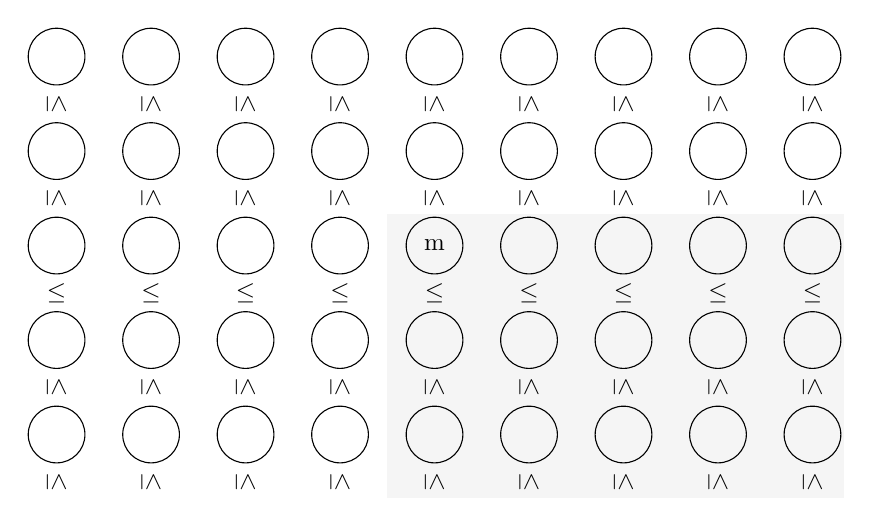
\begin{tikzpicture}[scale=1, every node/.style={scale=0.9}]
  \def\rows{5}
  \def\cols{9}
  \def\cellsize{1.2}

  \filldraw[fill=gray!30, opacity=0.25, draw=none]
    (5*\cellsize - 0.6, -3*\cellsize + 0.4) rectangle
    (9*\cellsize + 0.4, -6*\cellsize + 0.4);

  \foreach \i in {1,...,\rows} {
    \foreach \j in {1,...,\cols} {
      \pgfmathsetmacro\x{\j*\cellsize}
      \pgfmathsetmacro\y{-\i*\cellsize}
      \node[circle, draw, minimum size=8mm] (c\i\j) at (\x,\y) {};
      \ifnum\i=3
        \ifnum\j=5
          \node at (\x,\y) {m};
        \fi
        \node at (\x,\y - 0.6) {\( \leq \)};
      \else
        \node at (\x,\y - 0.6) [rotate=-90]  {\( \leq \)};
      \fi
    }
  }
\end{tikzpicture}